% Options for packages loaded elsewhere
\PassOptionsToPackage{unicode}{hyperref}
\PassOptionsToPackage{hyphens}{url}
\PassOptionsToPackage{dvipsnames,svgnames,x11names}{xcolor}
%
\documentclass[
  letterpaper,
  DIV=11,
  numbers=noendperiod]{scrreprt}

\usepackage{amsmath,amssymb}
\usepackage{iftex}
\ifPDFTeX
  \usepackage[T1]{fontenc}
  \usepackage[utf8]{inputenc}
  \usepackage{textcomp} % provide euro and other symbols
\else % if luatex or xetex
  \usepackage{unicode-math}
  \defaultfontfeatures{Scale=MatchLowercase}
  \defaultfontfeatures[\rmfamily]{Ligatures=TeX,Scale=1}
\fi
\usepackage{lmodern}
\ifPDFTeX\else  
    % xetex/luatex font selection
\fi
% Use upquote if available, for straight quotes in verbatim environments
\IfFileExists{upquote.sty}{\usepackage{upquote}}{}
\IfFileExists{microtype.sty}{% use microtype if available
  \usepackage[]{microtype}
  \UseMicrotypeSet[protrusion]{basicmath} % disable protrusion for tt fonts
}{}
\makeatletter
\@ifundefined{KOMAClassName}{% if non-KOMA class
  \IfFileExists{parskip.sty}{%
    \usepackage{parskip}
  }{% else
    \setlength{\parindent}{0pt}
    \setlength{\parskip}{6pt plus 2pt minus 1pt}}
}{% if KOMA class
  \KOMAoptions{parskip=half}}
\makeatother
\usepackage{xcolor}
\setlength{\emergencystretch}{3em} % prevent overfull lines
\setcounter{secnumdepth}{5}
% Make \paragraph and \subparagraph free-standing
\makeatletter
\ifx\paragraph\undefined\else
  \let\oldparagraph\paragraph
  \renewcommand{\paragraph}{
    \@ifstar
      \xxxParagraphStar
      \xxxParagraphNoStar
  }
  \newcommand{\xxxParagraphStar}[1]{\oldparagraph*{#1}\mbox{}}
  \newcommand{\xxxParagraphNoStar}[1]{\oldparagraph{#1}\mbox{}}
\fi
\ifx\subparagraph\undefined\else
  \let\oldsubparagraph\subparagraph
  \renewcommand{\subparagraph}{
    \@ifstar
      \xxxSubParagraphStar
      \xxxSubParagraphNoStar
  }
  \newcommand{\xxxSubParagraphStar}[1]{\oldsubparagraph*{#1}\mbox{}}
  \newcommand{\xxxSubParagraphNoStar}[1]{\oldsubparagraph{#1}\mbox{}}
\fi
\makeatother

\usepackage{color}
\usepackage{fancyvrb}
\newcommand{\VerbBar}{|}
\newcommand{\VERB}{\Verb[commandchars=\\\{\}]}
\DefineVerbatimEnvironment{Highlighting}{Verbatim}{commandchars=\\\{\}}
% Add ',fontsize=\small' for more characters per line
\usepackage{framed}
\definecolor{shadecolor}{RGB}{241,243,245}
\newenvironment{Shaded}{\begin{snugshade}}{\end{snugshade}}
\newcommand{\AlertTok}[1]{\textcolor[rgb]{0.68,0.00,0.00}{#1}}
\newcommand{\AnnotationTok}[1]{\textcolor[rgb]{0.37,0.37,0.37}{#1}}
\newcommand{\AttributeTok}[1]{\textcolor[rgb]{0.40,0.45,0.13}{#1}}
\newcommand{\BaseNTok}[1]{\textcolor[rgb]{0.68,0.00,0.00}{#1}}
\newcommand{\BuiltInTok}[1]{\textcolor[rgb]{0.00,0.23,0.31}{#1}}
\newcommand{\CharTok}[1]{\textcolor[rgb]{0.13,0.47,0.30}{#1}}
\newcommand{\CommentTok}[1]{\textcolor[rgb]{0.37,0.37,0.37}{#1}}
\newcommand{\CommentVarTok}[1]{\textcolor[rgb]{0.37,0.37,0.37}{\textit{#1}}}
\newcommand{\ConstantTok}[1]{\textcolor[rgb]{0.56,0.35,0.01}{#1}}
\newcommand{\ControlFlowTok}[1]{\textcolor[rgb]{0.00,0.23,0.31}{\textbf{#1}}}
\newcommand{\DataTypeTok}[1]{\textcolor[rgb]{0.68,0.00,0.00}{#1}}
\newcommand{\DecValTok}[1]{\textcolor[rgb]{0.68,0.00,0.00}{#1}}
\newcommand{\DocumentationTok}[1]{\textcolor[rgb]{0.37,0.37,0.37}{\textit{#1}}}
\newcommand{\ErrorTok}[1]{\textcolor[rgb]{0.68,0.00,0.00}{#1}}
\newcommand{\ExtensionTok}[1]{\textcolor[rgb]{0.00,0.23,0.31}{#1}}
\newcommand{\FloatTok}[1]{\textcolor[rgb]{0.68,0.00,0.00}{#1}}
\newcommand{\FunctionTok}[1]{\textcolor[rgb]{0.28,0.35,0.67}{#1}}
\newcommand{\ImportTok}[1]{\textcolor[rgb]{0.00,0.46,0.62}{#1}}
\newcommand{\InformationTok}[1]{\textcolor[rgb]{0.37,0.37,0.37}{#1}}
\newcommand{\KeywordTok}[1]{\textcolor[rgb]{0.00,0.23,0.31}{\textbf{#1}}}
\newcommand{\NormalTok}[1]{\textcolor[rgb]{0.00,0.23,0.31}{#1}}
\newcommand{\OperatorTok}[1]{\textcolor[rgb]{0.37,0.37,0.37}{#1}}
\newcommand{\OtherTok}[1]{\textcolor[rgb]{0.00,0.23,0.31}{#1}}
\newcommand{\PreprocessorTok}[1]{\textcolor[rgb]{0.68,0.00,0.00}{#1}}
\newcommand{\RegionMarkerTok}[1]{\textcolor[rgb]{0.00,0.23,0.31}{#1}}
\newcommand{\SpecialCharTok}[1]{\textcolor[rgb]{0.37,0.37,0.37}{#1}}
\newcommand{\SpecialStringTok}[1]{\textcolor[rgb]{0.13,0.47,0.30}{#1}}
\newcommand{\StringTok}[1]{\textcolor[rgb]{0.13,0.47,0.30}{#1}}
\newcommand{\VariableTok}[1]{\textcolor[rgb]{0.07,0.07,0.07}{#1}}
\newcommand{\VerbatimStringTok}[1]{\textcolor[rgb]{0.13,0.47,0.30}{#1}}
\newcommand{\WarningTok}[1]{\textcolor[rgb]{0.37,0.37,0.37}{\textit{#1}}}

\providecommand{\tightlist}{%
  \setlength{\itemsep}{0pt}\setlength{\parskip}{0pt}}\usepackage{longtable,booktabs,array}
\usepackage{calc} % for calculating minipage widths
% Correct order of tables after \paragraph or \subparagraph
\usepackage{etoolbox}
\makeatletter
\patchcmd\longtable{\par}{\if@noskipsec\mbox{}\fi\par}{}{}
\makeatother
% Allow footnotes in longtable head/foot
\IfFileExists{footnotehyper.sty}{\usepackage{footnotehyper}}{\usepackage{footnote}}
\makesavenoteenv{longtable}
\usepackage{graphicx}
\makeatletter
\newsavebox\pandoc@box
\newcommand*\pandocbounded[1]{% scales image to fit in text height/width
  \sbox\pandoc@box{#1}%
  \Gscale@div\@tempa{\textheight}{\dimexpr\ht\pandoc@box+\dp\pandoc@box\relax}%
  \Gscale@div\@tempb{\linewidth}{\wd\pandoc@box}%
  \ifdim\@tempb\p@<\@tempa\p@\let\@tempa\@tempb\fi% select the smaller of both
  \ifdim\@tempa\p@<\p@\scalebox{\@tempa}{\usebox\pandoc@box}%
  \else\usebox{\pandoc@box}%
  \fi%
}
% Set default figure placement to htbp
\def\fps@figure{htbp}
\makeatother

\KOMAoption{captions}{tableheading}
\makeatletter
\@ifpackageloaded{bookmark}{}{\usepackage{bookmark}}
\makeatother
\makeatletter
\@ifpackageloaded{caption}{}{\usepackage{caption}}
\AtBeginDocument{%
\ifdefined\contentsname
  \renewcommand*\contentsname{Table of contents}
\else
  \newcommand\contentsname{Table of contents}
\fi
\ifdefined\listfigurename
  \renewcommand*\listfigurename{List of Figures}
\else
  \newcommand\listfigurename{List of Figures}
\fi
\ifdefined\listtablename
  \renewcommand*\listtablename{List of Tables}
\else
  \newcommand\listtablename{List of Tables}
\fi
\ifdefined\figurename
  \renewcommand*\figurename{Figure}
\else
  \newcommand\figurename{Figure}
\fi
\ifdefined\tablename
  \renewcommand*\tablename{Table}
\else
  \newcommand\tablename{Table}
\fi
}
\@ifpackageloaded{float}{}{\usepackage{float}}
\floatstyle{ruled}
\@ifundefined{c@chapter}{\newfloat{codelisting}{h}{lop}}{\newfloat{codelisting}{h}{lop}[chapter]}
\floatname{codelisting}{Listing}
\newcommand*\listoflistings{\listof{codelisting}{List of Listings}}
\makeatother
\makeatletter
\makeatother
\makeatletter
\@ifpackageloaded{caption}{}{\usepackage{caption}}
\@ifpackageloaded{subcaption}{}{\usepackage{subcaption}}
\makeatother

\usepackage{bookmark}

\IfFileExists{xurl.sty}{\usepackage{xurl}}{} % add URL line breaks if available
\urlstyle{same} % disable monospaced font for URLs
\hypersetup{
  pdftitle={Introduction to R},
  pdfauthor={Dr Mehtap Hisarciklilar \& Dr Robert Riegler},
  colorlinks=true,
  linkcolor={blue},
  filecolor={Maroon},
  citecolor={Blue},
  urlcolor={Blue},
  pdfcreator={LaTeX via pandoc}}


\title{Introduction to R}
\author{Dr Mehtap Hisarciklilar \& Dr Robert Riegler}
\date{2025-01-20}

\begin{document}
\maketitle

\renewcommand*\contentsname{Table of contents}
{
\hypersetup{linkcolor=}
\setcounter{tocdepth}{2}
\tableofcontents
}

\bookmarksetup{startatroot}

\chapter*{Welcome!}\label{welcome}
\addcontentsline{toc}{chapter}{Welcome!}

\markboth{Welcome!}{Welcome!}

This workbook is created for the Introduction to R sessions at Coventry
University\footnote{The workshop series are organised by the School of
  EFA Economics Lab team in collaboration with the British Council
  funded project ``Strengthening Pathways into Employment: Female
  Students in Economics and Finance''.}.

organised by the School of EFA Economics Lab team in collaboration with
the British Council funded project ``Strengthening Pathways into
Employment: Female Students in Economics and Finance'' at Coventry
University.

It is written using Quarto on RStudio by

\textbf{Dr Mehtap Hisarciklilar}, Centre for Financial and Corporate
Integrity

\textbf{Dr Robert Riegler}, Aston University

\part{Session 1 Introduction to Data Analysis}

\chapter{Introduction to R}\label{introduction-to-r}

\section{R, R Studio and Quarto}\label{r-r-studio-and-quarto}

R is a very powerful statistical software that is becoming increasingly
popular. Being able to do data analysis using R will very likely
increase your employability.

\textbf{Warning: R is not like other apps that you have used! It
requires coding. You will need to practice regularly. There will be a
lot of struggle, but the result is worth it.}

We list below the apps that you will need to work with during the
sessions. You may install these on your computers. Alternatively, you
may use Coventry University's
\href{https://appsanywhere.coventry.ac.uk/}{Appsanywhere platform} to
get access. But you will find working with the app easier if it is
locally installed.

\begin{itemize}
\item
  We will be using \textbf{R} as the statistical analysis tool. For R
  documentations, support and download links, visit
  \href{https://www.r-project.org/}{the R Project for Statistical
  Computing}. R is freely available for Linux, MacOS and Windows.
  \textbf{Please download the version that matches your computer's
  operating system.}
\item
  To facilitate your work with R, we highly recommend to download and
  install the integrated development environment (IDE) \textbf{RStudio
  Desktop} from \href{https://posit.co/downloads/}{posit}. This platform
  will make it easier for you to write and run R code.
\item
  A final package that we highly recommend you to install is a
  publishing system, \textbf{Quarto}. You may use Quarto to produce
  documents in various formats (such as HTML, MS Word, PDF, PowerPoint,
  etc) while integrating your R code and output. You will easily have
  the option to change the format of your output as you desire. We will
  be using Quarto to produce documents in the third session of the
  series. Please visit \href{https://quarto.org/}{Quarto} for further
  information and download.

  \begin{itemize}
  \tightlist
  \item
    Once you download Quarto, you will have access to it through
    RStudio.
  \end{itemize}
\end{itemize}

RStudio has four main windows, that often have more than just one
purpose. Figure~\ref{fig-rstudio-windows} provides a brief description
of each RStudio window. We will use all of them during the sessions, but
the most important ones will be the console and the editor pane.

\begin{figure}

\centering{

\pandocbounded{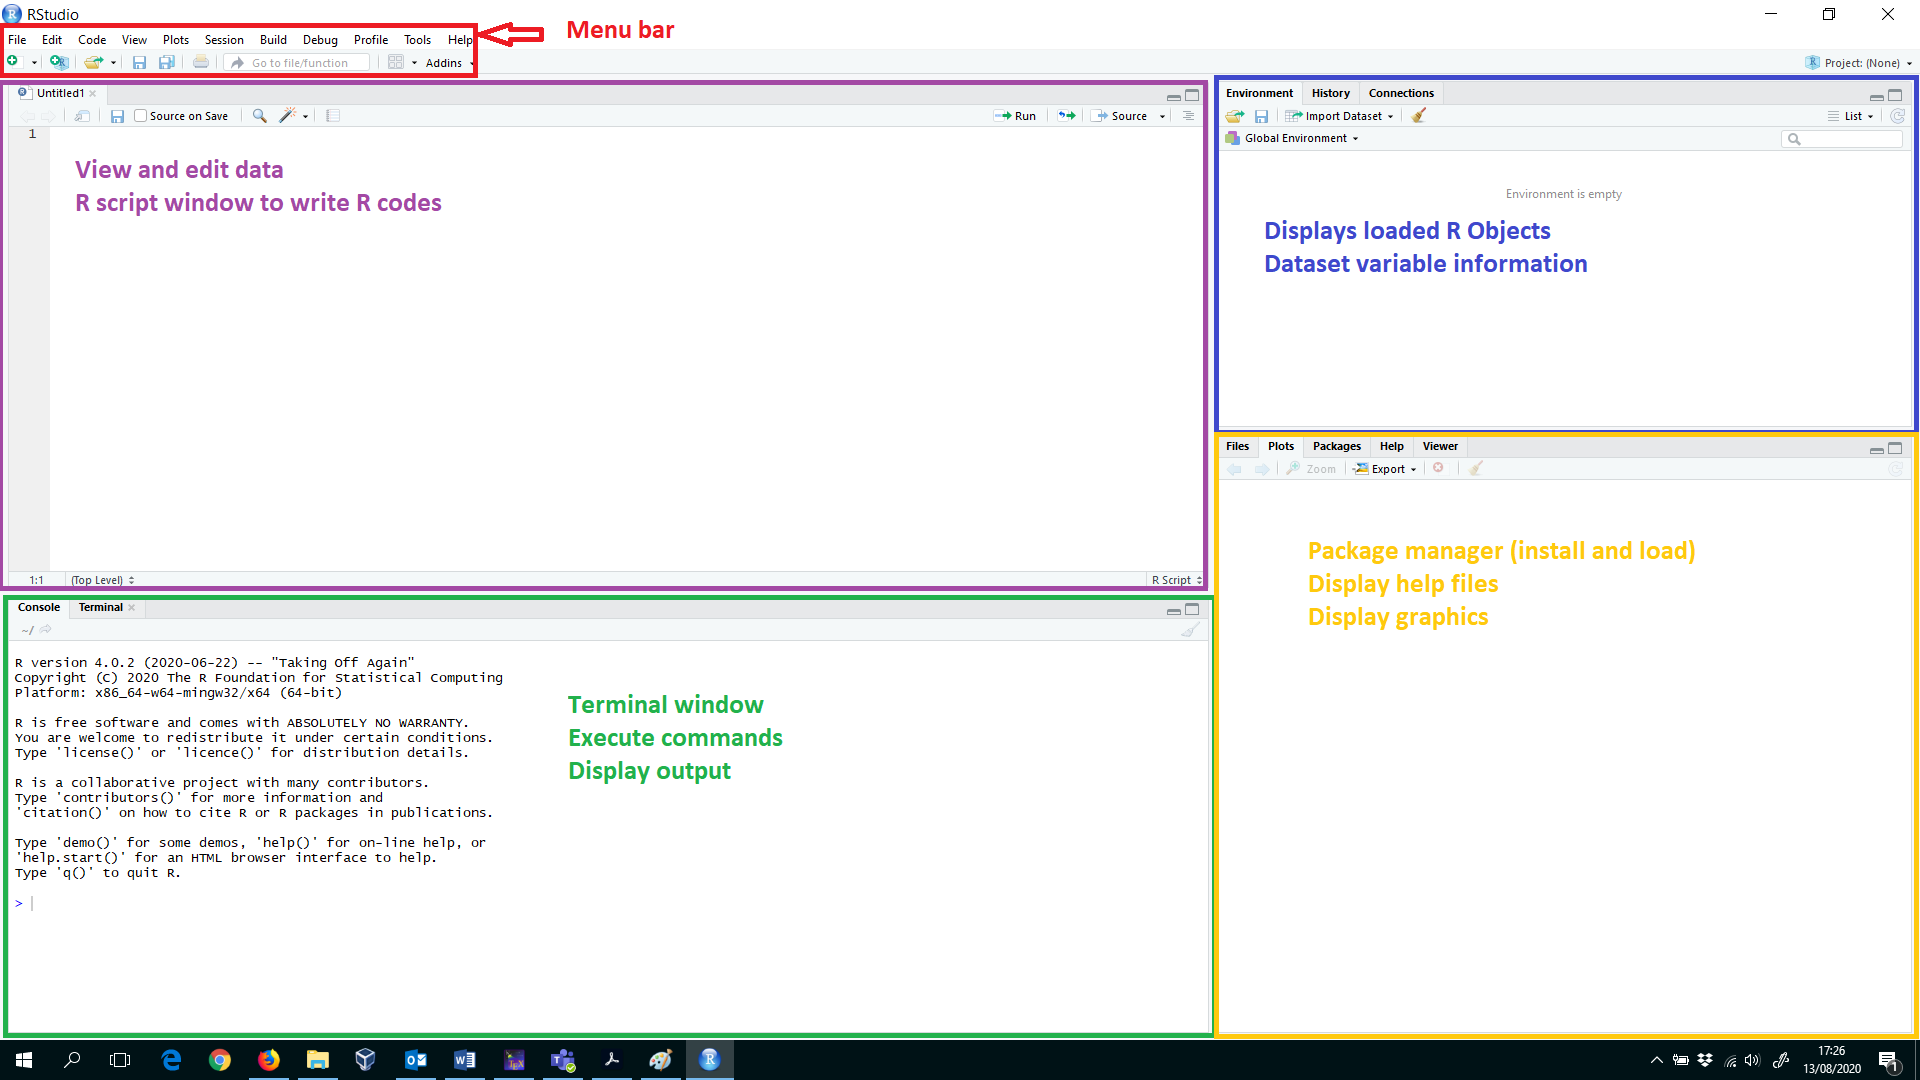
\includegraphics[keepaspectratio]{assets/images/introduction/rstudio.png}}

}

\caption{\label{fig-rstudio-windows}RStudio windows and their functions}

\end{figure}%

\section{File Organisation}\label{file-organisation}

\begin{itemize}
\item
  Create a folder for this workshop. This folder should include all
  material you download from
  \href{2025.03\%20--\%20Introduction\%20to\%20R\%20Software}{shared
  OneDrive folder}. Group files in sub-folders in a way that you can
  locate them easily. So for example, \texttt{Introduction-to-R} may be
  the name of the folder and then you may have sub-folders such as
  \texttt{data}, \texttt{R-scripts}, etc.
\item
  If you are using the computers in the lab, it may be best if you
  create a folder on your OneDrive account as you can easily access this
  at home and on-campus.
\item
  Before working on the data, set your working directory. R will save
  all files in there and, if you want to open a dataset, R will also
  look in there first. Select the folder you have created for R
  workshops.
\item
  Use
  \texttt{setwd(the\_address\_you\_would\_like\_to\_locate\_your\_work)}
  in the console to choose your work directory. You may alternatively do
  this through the menu:
\end{itemize}

\textbf{Session --\textgreater{} Set Working Directory --\textgreater{}
Choose Directory}

You will see the console printing this action, which may help you to
remember how to use the console next time.

\begin{itemize}
\tightlist
\item
  If you are unsure of in which folder your work is, type
  \texttt{getwd()} in the console and R will print the current location
  you are at.
\end{itemize}

\section{Getting Help}\label{getting-help}

If you should ever struggle with some of R's commands, a look into R's
help-files can be very helpful. To access the help file, you have to
type into the console window \texttt{?} and then the command name. For
example, if you want to know more about the command \texttt{getwd()},
type the following:

\begin{Shaded}
\begin{Highlighting}[]
\NormalTok{?}\FunctionTok{getwd}\NormalTok{()}
\end{Highlighting}
\end{Shaded}

\chapter{Basics of R}\label{basics-of-r}

\section{Using R as a calculator}\label{using-r-as-a-calculator}

You may use R as a calculator. Some examples are given below.

\begin{Shaded}
\begin{Highlighting}[]
\CommentTok{\# Addition}
\DecValTok{5} \SpecialCharTok{+} \DecValTok{4}
\end{Highlighting}
\end{Shaded}

\begin{verbatim}
[1] 9
\end{verbatim}

\begin{Shaded}
\begin{Highlighting}[]
\CommentTok{\# Subtraction}
\DecValTok{5} \SpecialCharTok{{-}} \DecValTok{4}
\end{Highlighting}
\end{Shaded}

\begin{verbatim}
[1] 1
\end{verbatim}

\begin{Shaded}
\begin{Highlighting}[]
\CommentTok{\# Multiplication}
\DecValTok{3} \SpecialCharTok{*} \DecValTok{6}
\end{Highlighting}
\end{Shaded}

\begin{verbatim}
[1] 18
\end{verbatim}

\begin{Shaded}
\begin{Highlighting}[]
\CommentTok{\# Division}
\DecValTok{10} \SpecialCharTok{/} \DecValTok{2}
\end{Highlighting}
\end{Shaded}

\begin{verbatim}
[1] 5
\end{verbatim}

\begin{Shaded}
\begin{Highlighting}[]
\CommentTok{\# Exponents}
\DecValTok{2}\SpecialCharTok{\^{}}\DecValTok{3}
\end{Highlighting}
\end{Shaded}

\begin{verbatim}
[1] 8
\end{verbatim}

\begin{Shaded}
\begin{Highlighting}[]
\CommentTok{\# Modulo}
\DecValTok{5} \SpecialCharTok{\%\%} \DecValTok{2}
\end{Highlighting}
\end{Shaded}

\begin{verbatim}
[1] 1
\end{verbatim}

\subsection{Basic Operators}\label{basic-operators}

\begin{longtable}[]{@{}ll@{}}
\toprule\noalign{}
\textbf{Operator} & \textbf{Description} \\
\midrule\noalign{}
\endhead
\bottomrule\noalign{}
\endlastfoot
\textbf{Arithmetic} & \\
\textbf{+} & Addition \\
\textbf{-} & Subtraction \\
\textbf{*} & Multiplication \\
\textbf{/} & Division \\
\textbf{\^{}} or \textbf{**} & Exponential \\
\textbf{\%\%} & Modulus \\
\textbf{\% / \%} & Integer Division \\
\textbf{Logic} & \\
\textbf{\textless{}} & Less than \\
\textbf{\textless=} & Less than or equal to \\
\textbf{\textgreater{}} & Greater than \\
\textbf{\textgreater=} & Greater than or equal to \\
\textbf{==} & Exactly equal to \\
\textbf{!=} & Not equal to \\
\textbf{!x} & Not x \\
\textbf{x \textbar{} y} & x OR y \\
\textbf{x \& y} & x AND y \\
\end{longtable}

\subsection{Order of operators}\label{order-of-operators}

\begin{itemize}
\item
  Parenthesis
\item
  Multiplication / division
\item
  Addition / subtraction
\item
  Multiplication has the same importance as division. Similarly,
  addition and subtraction are at the same level. When we need to decide
  between the two, we apply the operation that shows first from the left
  to the right.
\item
  Use of parentheses makes it easier to perform the correct operation
\item
  Can you guess the result of the following operation?

  \begin{itemize}
  \tightlist
  \item
    8 / 2 * ( 2 + 2)
  \end{itemize}
\end{itemize}

\begin{Shaded}
\begin{Highlighting}[]
\DecValTok{8} \SpecialCharTok{/} \DecValTok{2} \SpecialCharTok{*}\NormalTok{ ( }\DecValTok{2} \SpecialCharTok{+} \DecValTok{2}\NormalTok{)}
\end{Highlighting}
\end{Shaded}

\begin{verbatim}
[1] 16
\end{verbatim}

\begin{Shaded}
\begin{Highlighting}[]
\DecValTok{8} \SpecialCharTok{/} \DecValTok{2} \SpecialCharTok{*} \DecValTok{2} \SpecialCharTok{+} \DecValTok{2}
\end{Highlighting}
\end{Shaded}

\begin{verbatim}
[1] 10
\end{verbatim}

\begin{Shaded}
\begin{Highlighting}[]
\DecValTok{100} \SpecialCharTok{*} \DecValTok{2} \SpecialCharTok{+} \DecValTok{50} \SpecialCharTok{/} \DecValTok{2}
\end{Highlighting}
\end{Shaded}

\begin{verbatim}
[1] 225
\end{verbatim}

\begin{Shaded}
\begin{Highlighting}[]
\NormalTok{(}\DecValTok{100} \SpecialCharTok{*} \DecValTok{2}\NormalTok{) }\SpecialCharTok{+}\NormalTok{ (}\DecValTok{50} \SpecialCharTok{/} \DecValTok{2}\NormalTok{)}
\end{Highlighting}
\end{Shaded}

\begin{verbatim}
[1] 225
\end{verbatim}

\section{Storing information in
objects}\label{storing-information-in-objects}

R lets you save data by storing it inside an R \texttt{object}. An
object is a name that you can use to call up stored data.

\begin{Shaded}
\begin{Highlighting}[]
\NormalTok{a }\OtherTok{\textless{}{-}} \DecValTok{5}

\NormalTok{a}
\end{Highlighting}
\end{Shaded}

\begin{verbatim}
[1] 5
\end{verbatim}

\begin{Shaded}
\begin{Highlighting}[]
\NormalTok{a }\SpecialCharTok{+} \DecValTok{2}
\end{Highlighting}
\end{Shaded}

\begin{verbatim}
[1] 7
\end{verbatim}

In the example above, we store value of 5 under object \texttt{a}. We
then call the value stored under \texttt{a} and sum it with 2.

Note the use of \texttt{\textless{}} together with \texttt{-} . This
representation (\texttt{\textless{}-}) resembles a backward pointing
arrow, and it assigns the value 2 to the object \texttt{a}.

\begin{Shaded}
\begin{Highlighting}[]
\NormalTok{b\_vector }\OtherTok{\textless{}{-}} \DecValTok{1}\SpecialCharTok{:}\DecValTok{6}
\NormalTok{b\_vector}
\end{Highlighting}
\end{Shaded}

\begin{verbatim}
[1] 1 2 3 4 5 6
\end{verbatim}

\begin{Shaded}
\begin{Highlighting}[]
\DocumentationTok{\#\# [1] 1 2 3 4 5 6}
\end{Highlighting}
\end{Shaded}

In the above example, we create a vector, whose elements are numbers
from 1 to 6 and store it under b\_vector.

When you create an object, the object will appear in the environment
pane of RStudio (on the top right-hand-side of the R screen). This pane
will show you all of the objects you've created since opening RStudio.

\subsection{Naming of objects}\label{naming-of-objects}

Note the following;

\begin{itemize}
\item
  An object name cannot start with a number (for example, \texttt{2var}
  or \texttt{2\_var})
\item
  A name cannot use some special symbols, like \texttt{\^{}},
  \texttt{!}, \texttt{\$}, \texttt{@}, \texttt{+}, \texttt{-},
  \texttt{/}, or \texttt{*} . You may use \texttt{\_}
\item
  R is case-sensitive, so \texttt{name} and \texttt{Name} will refer to
  different objects
\item
  R will overwrite any previous information stored in an object without
  asking your confirmation. So, be careful while making changes.
\item
  You can see which object names you have already used by calling the
  function \texttt{ls}:

\begin{Shaded}
\begin{Highlighting}[]
\FunctionTok{ls}\NormalTok{()}
\end{Highlighting}
\end{Shaded}

\begin{verbatim}
[1] "a"        "b_vector"
\end{verbatim}

\begin{Shaded}
\begin{Highlighting}[]
\DocumentationTok{\#\# [1] "a"        "b\_vector"}
\end{Highlighting}
\end{Shaded}
\end{itemize}

\subsection{Naming conventions}\label{naming-conventions}

You may see the following styles for naming of variables:

\begin{itemize}
\tightlist
\item
  Camel case
\end{itemize}

Camel case variable naming is common in Javascipt. However, it is
considered as bad practise in R. Try to avoid this kind of naming.

\begin{Shaded}
\begin{Highlighting}[]
\NormalTok{bankAccount }\OtherTok{=} \DecValTok{100}
\end{Highlighting}
\end{Shaded}

\begin{itemize}
\tightlist
\item
  Use of dots
\end{itemize}

dot is used in variable names by many R users. However, try to avoid
this too because base R uses dots in function names
(\texttt{contrib.url()}) and class names (\texttt{data.frame}). Avoiding
dot in your variable names will help you avoid confusion, particularly
in the initial stages of your learning!

\begin{Shaded}
\begin{Highlighting}[]
\NormalTok{bank.account }\OtherTok{=} \DecValTok{100}
\end{Highlighting}
\end{Shaded}

\begin{itemize}
\tightlist
\item
  Snake case
\end{itemize}

Use of snake case is considered to be good practice. Try to follow this
approach.

\begin{Shaded}
\begin{Highlighting}[]
\NormalTok{bank\_account }\OtherTok{=} \DecValTok{100}
\end{Highlighting}
\end{Shaded}

Note that you may find different users of R having a preference towards
different styles. The recommendations above are from the ``Tidyverse
style guide'', which is available from
\url{https://style.tidyverse.org}.

Start your variable names with a lower case and reserve the capital
letter start for function names!

\subsection{Removing objects}\label{removing-objects}

You will see that the \texttt{Environment} window can quickly get
over-crowded while working interactively. You may remove the objects
that you no longer need. by \texttt{rm(object\_name\ )}

\begin{Shaded}
\begin{Highlighting}[]
\FunctionTok{rm}\NormalTok{(a)}
\end{Highlighting}
\end{Shaded}

If you have too many objects piled up and you would like to remove them
all, then you may type \texttt{rm(list\ =\ ls())}. This will fully clear
your environment.

\begin{Shaded}
\begin{Highlighting}[]
\FunctionTok{rm}\NormalTok{(}\AttributeTok{list =} \FunctionTok{ls}\NormalTok{())}
\end{Highlighting}
\end{Shaded}

\subsection{Example of using
variables}\label{example-of-using-variables}

Let us calculate the module mark for a student who got 65\% from
coursework and 53\% from exam. The weights for the coursework and exam
are, respectively, 25\% and 75\%.

\begin{Shaded}
\begin{Highlighting}[]
\CommentTok{\# let\textquotesingle{}s calculate module mark for a student}
\NormalTok{coursework }\OtherTok{\textless{}{-}} \DecValTok{65}
\NormalTok{exam }\OtherTok{\textless{}{-}} \DecValTok{53}
\NormalTok{module\_mark }\OtherTok{\textless{}{-}}\NormalTok{ coursework }\SpecialCharTok{*} \FloatTok{0.25} \SpecialCharTok{+}\NormalTok{ exam }\SpecialCharTok{*} \FloatTok{0.75}

\FunctionTok{print}\NormalTok{(module\_mark)}
\end{Highlighting}
\end{Shaded}

\begin{verbatim}
[1] 56
\end{verbatim}

\section{Datatypes in R}\label{datatypes-in-r}

\subsection{Numeric}\label{numeric}

Decimal numbers and integers are part of the numeric class in R.

\subsubsection{Decimal (floating point
values)}\label{decimal-floating-point-values}

\begin{Shaded}
\begin{Highlighting}[]
\NormalTok{decimal\_number }\OtherTok{\textless{}{-}} \FloatTok{2.2}
\end{Highlighting}
\end{Shaded}

\subsubsection{Integer}\label{integer}

\begin{Shaded}
\begin{Highlighting}[]
\NormalTok{i }\OtherTok{\textless{}{-}} \DecValTok{5}
\end{Highlighting}
\end{Shaded}

\subsection{Logical}\label{logical}

Boolean values (TRUE and FALSE) are part of the logical class in R.
These are written in capital letters.

\begin{Shaded}
\begin{Highlighting}[]
\NormalTok{t }\OtherTok{\textless{}{-}} \ConstantTok{TRUE}
\NormalTok{f }\OtherTok{\textless{}{-}} \ConstantTok{FALSE}
\end{Highlighting}
\end{Shaded}

\begin{Shaded}
\begin{Highlighting}[]
\NormalTok{t}
\end{Highlighting}
\end{Shaded}

\begin{verbatim}
[1] TRUE
\end{verbatim}

\begin{Shaded}
\begin{Highlighting}[]
\NormalTok{f}
\end{Highlighting}
\end{Shaded}

\begin{verbatim}
[1] FALSE
\end{verbatim}

\subsection{Characters}\label{characters}

Text (string) values are known as characters in R. You may use single or
double quotation to create a text (string).

\begin{Shaded}
\begin{Highlighting}[]
\NormalTok{message }\OtherTok{\textless{}{-}} \StringTok{"hello all!"}
\FunctionTok{print}\NormalTok{(message)}
\end{Highlighting}
\end{Shaded}

\begin{verbatim}
[1] "hello all!"
\end{verbatim}

\begin{Shaded}
\begin{Highlighting}[]
\NormalTok{an\_other\_message }\OtherTok{\textless{}{-}} \StringTok{\textquotesingle{}how are you?\textquotesingle{}}
\FunctionTok{print}\NormalTok{(an\_other\_message)}
\end{Highlighting}
\end{Shaded}

\begin{verbatim}
[1] "how are you?"
\end{verbatim}

\subsection{Checking data type
classes}\label{checking-data-type-classes}

We can use the \texttt{class()} function to check the data type of a
variable:

\begin{Shaded}
\begin{Highlighting}[]
\FunctionTok{class}\NormalTok{(decimal\_number)}
\end{Highlighting}
\end{Shaded}

\begin{verbatim}
[1] "numeric"
\end{verbatim}

\begin{Shaded}
\begin{Highlighting}[]
\FunctionTok{class}\NormalTok{(i)}
\end{Highlighting}
\end{Shaded}

\begin{verbatim}
[1] "numeric"
\end{verbatim}

\begin{Shaded}
\begin{Highlighting}[]
\FunctionTok{class}\NormalTok{(t)}
\end{Highlighting}
\end{Shaded}

\begin{verbatim}
[1] "logical"
\end{verbatim}

\begin{Shaded}
\begin{Highlighting}[]
\FunctionTok{class}\NormalTok{(f)}
\end{Highlighting}
\end{Shaded}

\begin{verbatim}
[1] "logical"
\end{verbatim}

\begin{Shaded}
\begin{Highlighting}[]
\FunctionTok{class}\NormalTok{(message)}
\end{Highlighting}
\end{Shaded}

\begin{verbatim}
[1] "character"
\end{verbatim}

\section{Scripts}\label{scripts}

You can create a draft of your code as you go by using an R
\emph{script}. An R script is just a plain text file that you save R
code in. You can open an R script in RStudio using the menu bar:

\emph{File --\textgreater{} New File --\textgreater{} R Script}

We will write and edit R code in a script. This will help create a
reproducible record of your work. When you're finished for the day, you
can save your script and then use it to rerun your entire analysis the
next day.

To save a script, click the scripts pane, and then go to \emph{File
--\textgreater{} Save As} in the menu bar.

\begin{itemize}
\item
  You can automatically execute a line of code in a script by clicking
  the Run button on the top right of the pane. R will run whichever line
  of code your cursor is on.
\item
  If you have a whole section highlighted, R will run the highlighted
  code.
\item
  You can run the entire script by clicking the Source button.
\item
  You can use Control + Return in your keyboard as a shortcut for the
  Run button. On Macs, that would be Command + Return.
\end{itemize}

\chapter{Importing and Viewing Data}\label{importing-and-viewing-data}

\section{Example: House Price Data}\label{example-house-price-data}

The data that we will be using in this session come from R's
\texttt{wooldridge} package, which includes 115 data sets from
``Introductory Econometrics: A Modern Approach, 7e'' by Jeffrey M.
Wooldridge''.

We will start by using \texttt{hprice2} data, which includes information
on 506 communities in the US Boston area. Below table provides a list of
variables that we will use:

\begin{longtable}[]{@{}ll@{}}
\toprule\noalign{}
Variable & Description \\
\midrule\noalign{}
\endhead
\bottomrule\noalign{}
\endlastfoot
price & Median housing price, \$ \\
crime & Crimes committed per capita \\
nox & Nitrogen Oxide in the air, in parts per million \\
stratio & Average student-teacher ratio of schools in the community \\
rooms & Average number of rooms in houses in the community \\
lprice & Logarithm of price \\
\end{longtable}

\section{Packages and libraries}\label{packages-and-libraries}

In order to access specialised data analysis tools in R, we will need to
install some R packages.

``An R \textbf{package} is a collection of functions, data, and
documentation that extends the capabilities of base R.

We will start by installing the \texttt{wooldridge} package. We require
this package to access the Wooldridge data sets, mentioned above.

\begin{Shaded}
\begin{Highlighting}[]
\CommentTok{\# install.packages("wooldridge")}
\end{Highlighting}
\end{Shaded}

To install \texttt{wooldridge} package, type the above line of code in
the console (without the \texttt{\#}), and then press enter to run it. R
will download the packages from CRAN and install them on to your
computer.

Once installed, you may use this package after loading it with the
\texttt{library()} function.

\begin{Shaded}
\begin{Highlighting}[]
\FunctionTok{library}\NormalTok{(wooldridge)}
\end{Highlighting}
\end{Shaded}

\section{Open data as an R object}\label{open-data-as-an-r-object}

The \texttt{hprice2} data that we will be using already comes in R
format within the \texttt{wooldridge} package. We can call it to our
environment by using the \texttt{data()} function.

\begin{Shaded}
\begin{Highlighting}[]
\FunctionTok{data}\NormalTok{(}\StringTok{"hprice2"}\NormalTok{)}
\end{Highlighting}
\end{Shaded}

Observe that \texttt{hprice2} is now added as an object to your
environment. We can use the \texttt{View} function to view it (Note the
capital V in \texttt{View}).Type the below line without the \texttt{\#}
in your console.

\begin{Shaded}
\begin{Highlighting}[]
\CommentTok{\# View(hprice2)}
\end{Highlighting}
\end{Shaded}

\section{Import Excel data into R}\label{import-excel-data-into-r}

Most data we work with are initially in Excel or in text (such as csv)
format. Importing data is one of the rare R commands that you can
proceed with using the menu. You may find the \texttt{Import\ Dataset}
button on the top right window and also under File menu. The
\texttt{hprice2} data is provided to you in Excel format. Try to import
it using \texttt{Import\ Dataset} but this time, in the opening window,
name the dataset as \texttt{df} under \texttt{Import\ Options} towards
the left bottom.

You will see that R executes the following three lines of code:

\begin{Shaded}
\begin{Highlighting}[]
\FunctionTok{library}\NormalTok{(readxl)}
\NormalTok{df }\OtherTok{\textless{}{-}} \FunctionTok{read\_excel}\NormalTok{(}\StringTok{"data/hprice2.xlsx"}\NormalTok{)}
\FunctionTok{View}\NormalTok{(df)}
\end{Highlighting}
\end{Shaded}

The first line call the library required; the second line reads the
Excel file and saves it under name \texttt{df} and the third line views
the newly imported data.

You may use \texttt{head()} and \texttt{tail()} functions to view,
respectively, the first few and the last few lines of the data.

\begin{Shaded}
\begin{Highlighting}[]
\CommentTok{\# View the first few observations of the data}
\FunctionTok{head}\NormalTok{(hprice2)}
\end{Highlighting}
\end{Shaded}

\begin{verbatim}
  price crime  nox rooms dist radial proptax stratio lowstat    lprice     lnox
1 24000 0.006 5.38  6.57 4.09      1    29.6    15.3    4.98 10.085809 1.682688
2 21599 0.027 4.69  6.42 4.97      2    24.2    17.8    9.14  9.980402 1.545433
3 34700 0.027 4.69  7.18 4.97      2    24.2    17.8    4.03 10.454495 1.545433
4 33400 0.032 4.58  7.00 6.06      3    22.2    18.7    2.94 10.416311 1.521699
5 36199 0.069 4.58  7.15 6.06      3    22.2    18.7    5.33 10.496787 1.521699
6 28701 0.030 4.58  6.43 6.06      3    22.2    18.7    5.21 10.264688 1.521699
  lproptax
1 5.690360
2 5.488938
3 5.488938
4 5.402678
5 5.402678
6 5.402678
\end{verbatim}

\begin{Shaded}
\begin{Highlighting}[]
\CommentTok{\# View the last few observations of the data}
\FunctionTok{tail}\NormalTok{(hprice2)}
\end{Highlighting}
\end{Shaded}

\begin{verbatim}
    price crime  nox rooms dist radial proptax stratio lowstat    lprice
501 16800 0.224 5.85  6.03 2.50      6    39.1    19.2   14.33  9.729135
502 22400 0.063 5.73  6.59 2.48      1    27.3    21.0    9.67 10.016816
503 20600 0.045 5.73  6.12 2.29      1    27.3    21.0    9.08  9.933046
504 23899 0.061 5.73  6.98 2.17      1    27.3    21.0    5.64 10.081592
505 22000 0.110 5.73  6.79 2.39      1    27.3    21.0    6.48  9.998797
506 11900 0.047 5.73  6.03 2.51      1    27.3    21.0    7.88  9.384294
        lnox lproptax
501 1.766442 5.968708
502 1.745715 5.609472
503 1.745715 5.609472
504 1.745715 5.609472
505 1.745715 5.609472
506 1.745715 5.609472
\end{verbatim}

\chapter{Calculating Summary
Statistics}\label{calculating-summary-statistics}

\begin{itemize}
\tightlist
\item
  We may use the \texttt{mean()} function to find the average value of a
  variable. For example, below, we find the average housing price:
\end{itemize}

\begin{Shaded}
\begin{Highlighting}[]
\CommentTok{\# Calculate the average price}
\FunctionTok{mean}\NormalTok{(hprice2}\SpecialCharTok{$}\NormalTok{price)}
\end{Highlighting}
\end{Shaded}

\begin{verbatim}
[1] 22511.51
\end{verbatim}

\begin{itemize}
\tightlist
\item
  Similarly \texttt{median()} function could be used to find the median.
\end{itemize}

\begin{Shaded}
\begin{Highlighting}[]
\CommentTok{\# Calculate the median price}
\FunctionTok{median}\NormalTok{(hprice2}\SpecialCharTok{$}\NormalTok{price)}
\end{Highlighting}
\end{Shaded}

\begin{verbatim}
[1] 21200
\end{verbatim}

\begin{itemize}
\tightlist
\item
  Use \texttt{sd()} for standard deviation
\end{itemize}

\begin{Shaded}
\begin{Highlighting}[]
\CommentTok{\# Calculate the standard deviation of price}
\FunctionTok{sd}\NormalTok{(hprice2}\SpecialCharTok{$}\NormalTok{price)}
\end{Highlighting}
\end{Shaded}

\begin{verbatim}
[1] 9208.856
\end{verbatim}

You may wonder why we add \texttt{hprice2\$} in front of every variable.
The reason is that R can store more than one data frame, matrix, list,
vector etc., at the same time, so the prefix \texttt{hprice2\$} is
necessary to avoid ambiguity and ensure that we are working with
variables in the \texttt{hprice2} data. Think of \texttt{hprice2\$} as
an address where e.g.~the variable \texttt{price} stays. If you have
loaded another data frame that contains a \texttt{price} variable, R
would know that we want to use the variable from the hprice2 data set
and not from the other data frame. There are library packages that can
facilitate the process, however, these are beyond the scope of this
workshop.

In addition to mean and median, we may be interested with the minimum
and maximum values. In that case, we can use the \texttt{summary()}
function to ask for a full set of summary statistics. (Please note that
\texttt{summary()} function does not report the standard deviation. You
will need to use the \texttt{sd()} function for that).

\begin{Shaded}
\begin{Highlighting}[]
\CommentTok{\# Summary statistics for price}
\FunctionTok{summary}\NormalTok{(hprice2}\SpecialCharTok{$}\NormalTok{price)}
\end{Highlighting}
\end{Shaded}

\begin{verbatim}
   Min. 1st Qu.  Median    Mean 3rd Qu.    Max. 
   5000   16850   21200   22512   24999   50001 
\end{verbatim}

Again, note the use of \texttt{hprice2\$} above.

We can provide the name of the data set as an argument in the
\texttt{summary()} function to get summary statistics for all variables
in the data.

\begin{Shaded}
\begin{Highlighting}[]
\CommentTok{\# summary statistics for all variables}
\FunctionTok{summary}\NormalTok{(hprice2)}
\end{Highlighting}
\end{Shaded}

\begin{verbatim}
     price           crime              nox           rooms      
 Min.   : 5000   Min.   : 0.0060   Min.   :3.85   Min.   :3.560  
 1st Qu.:16850   1st Qu.: 0.0820   1st Qu.:4.49   1st Qu.:5.883  
 Median :21200   Median : 0.2565   Median :5.38   Median :6.210  
 Mean   :22512   Mean   : 3.6115   Mean   :5.55   Mean   :6.284  
 3rd Qu.:24999   3rd Qu.: 3.6770   3rd Qu.:6.24   3rd Qu.:6.620  
 Max.   :50001   Max.   :88.9760   Max.   :8.71   Max.   :8.780  
      dist            radial          proptax         stratio     
 Min.   : 1.130   Min.   : 1.000   Min.   :18.70   Min.   :12.60  
 1st Qu.: 2.100   1st Qu.: 4.000   1st Qu.:27.90   1st Qu.:17.40  
 Median : 3.210   Median : 5.000   Median :33.00   Median :19.10  
 Mean   : 3.796   Mean   : 9.549   Mean   :40.82   Mean   :18.46  
 3rd Qu.: 5.188   3rd Qu.:24.000   3rd Qu.:66.60   3rd Qu.:20.20  
 Max.   :12.130   Max.   :24.000   Max.   :71.10   Max.   :22.00  
    lowstat           lprice            lnox          lproptax    
 Min.   : 1.730   Min.   : 8.517   Min.   :1.348   Min.   :5.231  
 1st Qu.: 6.923   1st Qu.: 9.732   1st Qu.:1.502   1st Qu.:5.631  
 Median :11.360   Median : 9.962   Median :1.683   Median :5.799  
 Mean   :12.701   Mean   : 9.941   Mean   :1.693   Mean   :5.931  
 3rd Qu.:17.058   3rd Qu.:10.127   3rd Qu.:1.831   3rd Qu.:6.501  
 Max.   :39.070   Max.   :10.820   Max.   :2.164   Max.   :6.567  
\end{verbatim}

And finally, if we may want to have summary statistics only for a
selection of variables, for example, \texttt{price}, \texttt{nox}, and
\texttt{crime}.

\begin{Shaded}
\begin{Highlighting}[]
\CommentTok{\# summary statistics for a selection of variables:}
\FunctionTok{summary}\NormalTok{(hprice2[, }\FunctionTok{c}\NormalTok{(}\StringTok{"price"}\NormalTok{, }\StringTok{"nox"}\NormalTok{, }\StringTok{"crime"}\NormalTok{)])}
\end{Highlighting}
\end{Shaded}

\begin{verbatim}
     price            nox           crime        
 Min.   : 5000   Min.   :3.85   Min.   : 0.0060  
 1st Qu.:16850   1st Qu.:4.49   1st Qu.: 0.0820  
 Median :21200   Median :5.38   Median : 0.2565  
 Mean   :22512   Mean   :5.55   Mean   : 3.6115  
 3rd Qu.:24999   3rd Qu.:6.24   3rd Qu.: 3.6770  
 Max.   :50001   Max.   :8.71   Max.   :88.9760  
\end{verbatim}

We may calculate the covariance or correlation between the variables
using the \texttt{cov()} and \texttt{cor()} functions:

\begin{Shaded}
\begin{Highlighting}[]
\CommentTok{\# Covariance between price and crime}
\FunctionTok{cov}\NormalTok{(hprice2}\SpecialCharTok{$}\NormalTok{price, hprice2}\SpecialCharTok{$}\NormalTok{crime)}
\end{Highlighting}
\end{Shaded}

\begin{verbatim}
[1] -30686.87
\end{verbatim}

\begin{Shaded}
\begin{Highlighting}[]
\CommentTok{\# Correlation between price and crime}
\FunctionTok{cor}\NormalTok{(hprice2}\SpecialCharTok{$}\NormalTok{price, hprice2}\SpecialCharTok{$}\NormalTok{crime)}
\end{Highlighting}
\end{Shaded}

\begin{verbatim}
[1] -0.3879191
\end{verbatim}

\chapter{Labeling Variables}\label{labeling-variables}

There are alternative packages which could be used to label variables.
We will be using the \texttt{Hmisc} package. Remember to install this
package and call the library by running the code below (without the
\texttt{\#}):

\begin{Shaded}
\begin{Highlighting}[]
\CommentTok{\# install.packages("Hmisc") \# to label variables}
\FunctionTok{library}\NormalTok{(Hmisc)}
\end{Highlighting}
\end{Shaded}

\begin{verbatim}

Attaching package: 'Hmisc'
\end{verbatim}

\begin{verbatim}
The following objects are masked from 'package:base':

    format.pval, units
\end{verbatim}

We are ready to label our variables:

\begin{Shaded}
\begin{Highlighting}[]
\CommentTok{\# label variables}
\FunctionTok{label}\NormalTok{(hprice2}\SpecialCharTok{$}\NormalTok{price) }\OtherTok{\textless{}{-}} \StringTok{"Median housing price, $"}
\FunctionTok{label}\NormalTok{(hprice2}\SpecialCharTok{$}\NormalTok{crime) }\OtherTok{\textless{}{-}} \StringTok{"Crimes committed per capita"}
\FunctionTok{label}\NormalTok{(hprice2}\SpecialCharTok{$}\NormalTok{nox) }\OtherTok{\textless{}{-}} \StringTok{"Nitrogen Oxide in the air, in parts per million"}
\FunctionTok{label}\NormalTok{(hprice2}\SpecialCharTok{$}\NormalTok{stratio) }\OtherTok{\textless{}{-}} \StringTok{"Average student{-}teacher ratio of schools in the community"}
\FunctionTok{label}\NormalTok{(hprice2}\SpecialCharTok{$}\NormalTok{rooms) }\OtherTok{\textless{}{-}} \StringTok{"Average number of rooms in houses in the community"}
\end{Highlighting}
\end{Shaded}

\chapter{Basic Plots of Data}\label{basic-plots-of-data}

In Session 2 of this workshop, we will be using \texttt{ggplot2} for
data visualisation in R, which produces better-looking plots. For the
moment, below are a few examples of what we can do with base R (with
base R, we refer to the operations of R that could be done without
installing or calling additional libraries).

\textbf{Scatter plot}

We may use scatter plots to depict the relationship between two
variables. In the example below, we are depicting the relationship
between housing price and crime. You may read the
\texttt{\textasciitilde{}} between the two variables as
\emph{approximated by}. So here, price is approximated by crime.

\begin{Shaded}
\begin{Highlighting}[]
\CommentTok{\# scatterplot showing the relationship between price and crimes }
\FunctionTok{plot}\NormalTok{(hprice2}\SpecialCharTok{$}\NormalTok{price }\SpecialCharTok{\textasciitilde{}}\NormalTok{ hprice2}\SpecialCharTok{$}\NormalTok{crime)}
\end{Highlighting}
\end{Shaded}

\pandocbounded{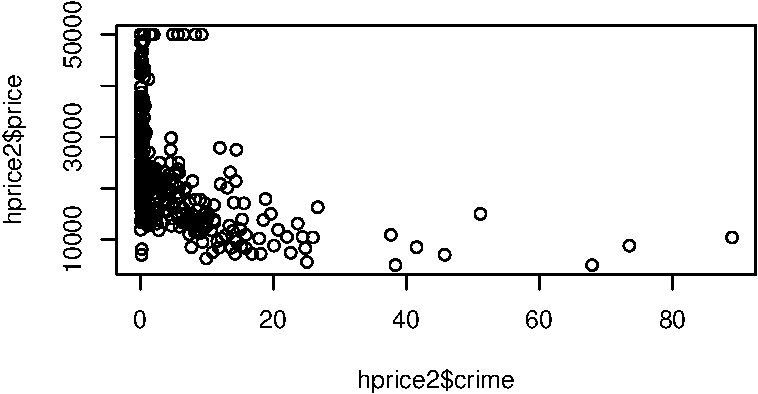
\includegraphics[keepaspectratio]{plotting-variables_files/figure-pdf/unnamed-chunk-2-1.pdf}}

We may add more informative titles to our axes and also provide a
general title for the plot:

\begin{Shaded}
\begin{Highlighting}[]
\CommentTok{\# scatterplot showing the relationship between price and crimes }
\FunctionTok{plot}\NormalTok{(hprice2}\SpecialCharTok{$}\NormalTok{price }\SpecialCharTok{\textasciitilde{}}\NormalTok{ hprice2}\SpecialCharTok{$}\NormalTok{crime, }
     \AttributeTok{xlab =} \StringTok{"Crimes committed per capita"}\NormalTok{, }
     \AttributeTok{ylab =} \StringTok{"Median housing price, $"}\NormalTok{, }
     \AttributeTok{main =} \StringTok{"Negative effect of crime on housing price"}\NormalTok{)}
\end{Highlighting}
\end{Shaded}

\pandocbounded{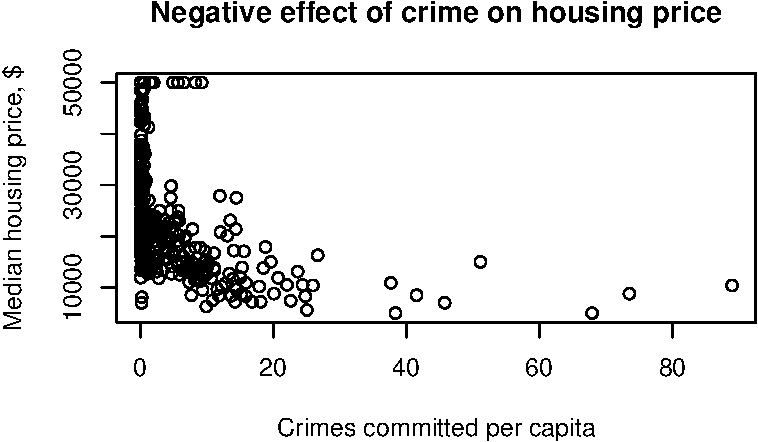
\includegraphics[keepaspectratio]{plotting-variables_files/figure-pdf/unnamed-chunk-3-1.pdf}}

As expected, there is a negative relationship between the crime rates in
a location and the median house prices in that location.

In the following pages, we will be estimating regresions to model the
houseing price with a set of independent variables. Before moving on to
regression analysis, it is good practice to get to know our dependent
variable. A histogram will reveal its distribution.

\textbf{Histogram}

Below, we provide histograms of \texttt{price} and \texttt{lprice}
(logarithmic price). Which one should we use in our regression?

\begin{Shaded}
\begin{Highlighting}[]
\CommentTok{\# Histogram of price and logarithmic price}
\FunctionTok{hist}\NormalTok{(hprice2}\SpecialCharTok{$}\NormalTok{price, }
     \AttributeTok{xlab =} \StringTok{"Median housing price, $"}\NormalTok{, }
     \AttributeTok{main =} \StringTok{"Histogram of median housing price, $"}\NormalTok{)}
\end{Highlighting}
\end{Shaded}

\pandocbounded{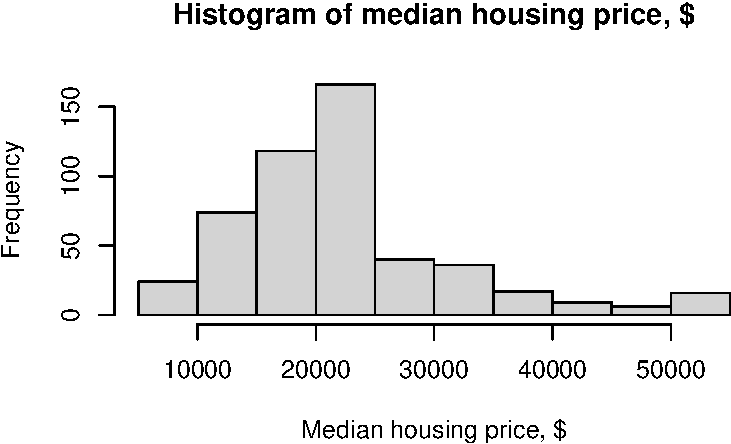
\includegraphics[keepaspectratio]{plotting-variables_files/figure-pdf/unnamed-chunk-4-1.pdf}}

\begin{Shaded}
\begin{Highlighting}[]
\FunctionTok{hist}\NormalTok{(hprice2}\SpecialCharTok{$}\NormalTok{lprice, }
     \AttributeTok{xlab =} \StringTok{"Logarithm of median housing price, $"}\NormalTok{, }
     \AttributeTok{main =} \StringTok{"Logarithm of median housing price, $"}\NormalTok{)}
\end{Highlighting}
\end{Shaded}

\pandocbounded{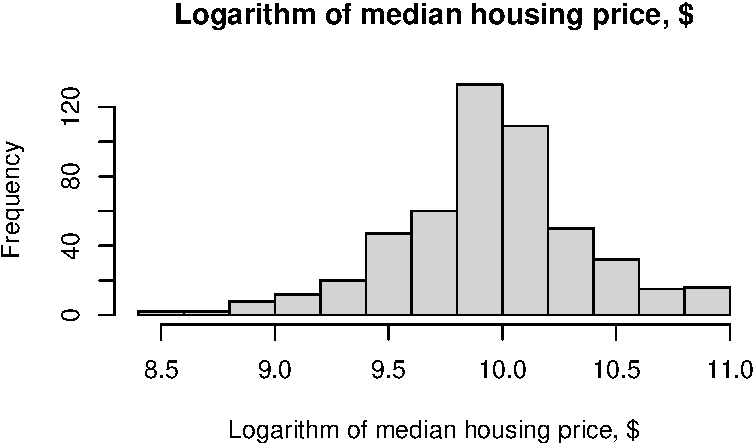
\includegraphics[keepaspectratio]{plotting-variables_files/figure-pdf/unnamed-chunk-5-1.pdf}}

\chapter{OLS Regression}\label{ols-regression}

We will start with a simple regression relating logarithmic house prices
with crime. Below, we will name and store this regression as
\texttt{model\_1}. Note that you may provide any name as you wish, as
long as it does not clash with the naming conventions. For example,
while \texttt{model\_1} is OK, \texttt{1\_model} is not possible.

\begin{Shaded}
\begin{Highlighting}[]
\CommentTok{\# Regression}
\NormalTok{model\_1 }\OtherTok{\textless{}{-}} \FunctionTok{lm}\NormalTok{(lprice }\SpecialCharTok{\textasciitilde{}}\NormalTok{ crime, }\AttributeTok{data =}\NormalTok{ hprice2)}
\FunctionTok{summary}\NormalTok{(model\_1)}
\end{Highlighting}
\end{Shaded}

\begin{verbatim}

Call:
lm(formula = lprice ~ crime, data = hprice2)

Residuals:
    Min      1Q  Median      3Q     Max 
-1.1736 -0.2041 -0.0301  0.1750  1.4538 

Coefficients:
             Estimate Std. Error t value Pr(>|t|)    
(Intercept) 10.031818   0.016786  597.63   <2e-16 ***
crime       -0.025131   0.001803  -13.94   <2e-16 ***
---
Signif. codes:  0 '***' 0.001 '**' 0.01 '*' 0.05 '.' 0.1 ' ' 1

Residual standard error: 0.348 on 504 degrees of freedom
Multiple R-squared:  0.2783,    Adjusted R-squared:  0.2768 
F-statistic: 194.3 on 1 and 504 DF,  p-value: < 2.2e-16
\end{verbatim}

\begin{itemize}
\item
  The R function we use for linear regression is \texttt{lm}, which
  stands for \emph{linear model}.
\item
  The regression equation we are estimating is given by
  \texttt{lprice\ \textasciitilde{}\ crime}, where \texttt{price} is
  approximated by \texttt{crime}.
\item
  \texttt{data\ =\ hprice2} refers to the hprice2 data we are using
\item
  \texttt{summary(model\_1)} is a separate line of command, which asks R
  to provide the summary estimation results.
\end{itemize}

We may add another independent variable in the model by using a
\texttt{+} sign. This time it is saved under name \texttt{model\_2}.

\begin{Shaded}
\begin{Highlighting}[]
\NormalTok{model\_2 }\OtherTok{\textless{}{-}} \FunctionTok{lm}\NormalTok{(lprice }\SpecialCharTok{\textasciitilde{}}\NormalTok{ crime }\SpecialCharTok{+}\NormalTok{ nox, }\AttributeTok{data =}\NormalTok{ hprice2)}
\FunctionTok{summary}\NormalTok{(model\_2)}
\end{Highlighting}
\end{Shaded}

\begin{verbatim}

Call:
lm(formula = lprice ~ crime + nox, data = hprice2)

Residuals:
     Min       1Q   Median       3Q      Max 
-1.08309 -0.18979 -0.05017  0.16518  1.10231 

Coefficients:
             Estimate Std. Error t value Pr(>|t|)    
(Intercept) 10.689699   0.074846 142.822   <2e-16 ***
crime       -0.018140   0.001847  -9.822   <2e-16 ***
nox         -0.123091   0.013696  -8.987   <2e-16 ***
---
Signif. codes:  0 '***' 0.001 '**' 0.01 '*' 0.05 '.' 0.1 ' ' 1

Residual standard error: 0.3234 on 503 degrees of freedom
Multiple R-squared:  0.3781,    Adjusted R-squared:  0.3756 
F-statistic: 152.9 on 2 and 503 DF,  p-value: < 2.2e-16
\end{verbatim}

Let us add two mode independent variables under name \texttt{model\_3}:

\begin{Shaded}
\begin{Highlighting}[]
\NormalTok{model\_3 }\OtherTok{\textless{}{-}} \FunctionTok{lm}\NormalTok{(lprice }\SpecialCharTok{\textasciitilde{}}\NormalTok{ crime }\SpecialCharTok{+}\NormalTok{ nox }\SpecialCharTok{+}\NormalTok{ stratio }\SpecialCharTok{+}\NormalTok{ rooms, }
              \AttributeTok{data =}\NormalTok{ hprice2)}
\FunctionTok{summary}\NormalTok{(model\_3)}
\end{Highlighting}
\end{Shaded}

\begin{verbatim}

Call:
lm(formula = lprice ~ crime + nox + stratio + rooms, data = hprice2)

Residuals:
     Min       1Q   Median       3Q      Max 
-0.87500 -0.12789  0.00664  0.11087  1.35514 

Coefficients:
             Estimate Std. Error t value Pr(>|t|)    
(Intercept)  9.653725   0.187981  51.355  < 2e-16 ***
crime       -0.013143   0.001450  -9.065  < 2e-16 ***
nox         -0.078260   0.010751  -7.279 1.31e-12 ***
stratio     -0.042702   0.005568  -7.670 9.04e-14 ***
rooms        0.247830   0.017289  14.334  < 2e-16 ***
---
Signif. codes:  0 '***' 0.001 '**' 0.01 '*' 0.05 '.' 0.1 ' ' 1

Residual standard error: 0.2465 on 501 degrees of freedom
Multiple R-squared:   0.64, Adjusted R-squared:  0.6371 
F-statistic: 222.6 on 4 and 501 DF,  p-value: < 2.2e-16
\end{verbatim}

We may want to save the residuals or predictions after estimating an OLS
model.

\begin{itemize}
\tightlist
\item
  Use \texttt{predict()} to store the predictions for the dependent
  variable.
\end{itemize}

Can you tell the difference between the two lines below?

\begin{Shaded}
\begin{Highlighting}[]
\NormalTok{price\_hat }\OtherTok{\textless{}{-}} \FunctionTok{predict}\NormalTok{(model\_3)}

\NormalTok{hprice2}\SpecialCharTok{$}\NormalTok{lprice\_hat }\OtherTok{\textless{}{-}} \FunctionTok{predict}\NormalTok{(model\_3)}
\end{Highlighting}
\end{Shaded}

In the first one predictions are saved under a separate object of its
own while the second line saves these as a variable in our
\texttt{hprice2} data.

\begin{itemize}
\tightlist
\item
  Use \texttt{rediduals} to store the residuals of the model.
\end{itemize}

\begin{Shaded}
\begin{Highlighting}[]
\CommentTok{\# Saving residuals of model\_3}
\NormalTok{resid\_3 }\OtherTok{\textless{}{-}} \FunctionTok{residuals}\NormalTok{(model\_3)}
\end{Highlighting}
\end{Shaded}

Let us view the newly created \texttt{lprice\_hat} variable. We can do
this by viewing the whole data set:

\begin{Shaded}
\begin{Highlighting}[]
\CommentTok{\# View the newly created predicted price variable {-} whole data}
\CommentTok{\#View(hprice2)}
\end{Highlighting}
\end{Shaded}

It is difficult to compare the actual and predicted value columns above.
We may ask R to view only a selection of variable rather than the full
data.

\begin{Shaded}
\begin{Highlighting}[]
\CommentTok{\# Create a subset of variables and then view them}
\NormalTok{subset }\OtherTok{\textless{}{-}}\NormalTok{ hprice2[, }\FunctionTok{c}\NormalTok{(}\StringTok{"lprice"}\NormalTok{, }\StringTok{"lprice\_hat"}\NormalTok{)]}
\CommentTok{\#View(subset)}

\CommentTok{\# Combining the two lines under one }
\CommentTok{\#View(hprice2[, c("lprice", "lprice\_hat")])}
\end{Highlighting}
\end{Shaded}

Finally, we may use a summary table to present results of the three
models together. We use the \texttt{stargazer} package for that.

\begin{Shaded}
\begin{Highlighting}[]
\CommentTok{\#install.packages("stargazer")}
\FunctionTok{library}\NormalTok{(stargazer)}
\end{Highlighting}
\end{Shaded}

\begin{verbatim}

Please cite as: 
\end{verbatim}

\begin{verbatim}
 Hlavac, Marek (2022). stargazer: Well-Formatted Regression and Summary Statistics Tables.
\end{verbatim}

\begin{verbatim}
 R package version 5.2.3. https://CRAN.R-project.org/package=stargazer 
\end{verbatim}

\begin{Shaded}
\begin{Highlighting}[]
\CommentTok{\# Summarising the three model estimates under one table}
\FunctionTok{stargazer}\NormalTok{(model\_1, model\_2, model\_3, }\AttributeTok{type =} \StringTok{"text"}\NormalTok{)}
\end{Highlighting}
\end{Shaded}

\begin{verbatim}

==============================================================================================
                                               Dependent variable:                            
                    --------------------------------------------------------------------------
                                                      lprice                                  
                              (1)                      (2)                      (3)           
----------------------------------------------------------------------------------------------
crime                      -0.025***                -0.018***                -0.013***        
                            (0.002)                  (0.002)                  (0.001)         
                                                                                              
nox                                                 -0.123***                -0.078***        
                                                     (0.014)                  (0.011)         
                                                                                              
stratio                                                                      -0.043***        
                                                                              (0.006)         
                                                                                              
rooms                                                                         0.248***        
                                                                              (0.017)         
                                                                                              
Constant                   10.032***                10.690***                 9.654***        
                            (0.017)                  (0.075)                  (0.188)         
                                                                                              
----------------------------------------------------------------------------------------------
Observations                  506                      506                      506           
R2                           0.278                    0.378                    0.640          
Adjusted R2                  0.277                    0.376                    0.637          
Residual Std. Error     0.348 (df = 504)         0.323 (df = 503)         0.247 (df = 501)    
F Statistic         194.303*** (df = 1; 504) 152.911*** (df = 2; 503) 222.623*** (df = 4; 501)
==============================================================================================
Note:                                                              *p<0.1; **p<0.05; ***p<0.01
\end{verbatim}

\chapter{Student Activity}\label{student-activity}

Work on the following tasks on your own or with a person sitting next to
you.

\begin{enumerate}
\def\labelenumi{\arabic{enumi}.}
\item
  Clear the environment
\item
  Create a new project called \texttt{birth-weight}. You may do this
  either through the File menu or the button on the top right center of
  your screen.
\item
  Import the \texttt{bweight} Excel data into R.
\item
  Below are the labels of the variables. Assign these to each of the
  correponding variable in data.

  \begin{longtable}[]{@{}ll@{}}
  \toprule\noalign{}
  Variable & Label \\
  \midrule\noalign{}
  \endhead
  \bottomrule\noalign{}
  \endlastfoot
  bwght & baby's birth weight, in grams \\
  mage & mother's age \\
  cigs & average number of cigarettes smoked per day \\
  male & dummy variable equal to 1 if baby is a male \\
  \end{longtable}
\item
  Provide summary statistics for the variables.
\item
  Calculate the standard deviation for the \texttt{bwght} variable.
\item
  Estimate a regression model which explains the \texttt{bwght} with the
  mother's age, smoking behaviour, and the baby's gender.
\item
  Using the model you estimated, predict the baby's birth weight for the
  individuals in the sample.
\end{enumerate}




\end{document}
